% 2017
% Guillermo Aguilar.
% 
\documentclass[10pt]{beamer}
\mode<presentation>
{
  \usetheme{CambridgeUS}
  \setbeamercovered{}
  % or whatever (possibly just delete it)
}
\setbeamertemplate{navigation symbols}{}%remove navigation symbols

\setbeamertemplate{itemize items}[default]
\setbeamertemplate{enumerate items}[default]

%\usefonttheme{professionalfonts}
\usepackage{listings}
\usepackage{times}
\usepackage{tikz}
\usepackage{amsmath}
\usepackage{verbatim}
\usetikzlibrary{arrows,shapes}
\graphicspath{{figures/}}
\usepackage[english]{babel}
\usepackage{mathtools}
\usepackage{tabularx}
\usepackage{graphicx,color,psfrag}
\usepackage{verbatimbox}
\usepackage{multirow}
\usepackage{changepage}



\title
{Statistics of Signal Detection Models}

\subtitle{usings GLMs in R} % (optional)

\author{Guillermo Aguilar}

\institute[TU Berlin] % (optional, but mostly needed)
{Technische Universit\"at Berlin}

\date[ECVP 2017]{August 27th, 2017}
\titlegraphic{\hfill \includegraphics[scale=0.3]{figs/TUlogo.pdf}}
\subject{Signal Detection Theory}

\begin{document}
%%
\begin{frame}
  \titlepage
\end{frame}

%%
\begin{frame}{Goal}
\begin{center}
Learn to analyze the most common experimental designs \\
in the framework of Signal Detection Theory using GLMs  in R
\end{center}
\end{frame}

%%
\begin{frame}
\tableofcontents
\end{frame}

%%
\begin{frame}{Resources}

\textbf{Knoblauch \& Maloney (2012). Modeling Psychophysical Data in R}\\
\vspace{10pt}
\textbf{Psychophysics}
\begin{itemize}
\item Kingdom \& Prins (2010). Psychophysics: A practical introduction.
\item Gescheider (1997). Psychophysics: The Fundamentals
\end{itemize}

\textbf{Signal detection theory}
\begin{itemize}
\item Wickens (2002). Elementary Signal Detection Theory.
\item McNicol (2005). A premier of Signal Detection Theory
\item Macmillian \& Creelman (2005). Detection Theory. A User's Guide
\item Green \& Swets (1966). Signal Detection Theory and Psychophysics.
\end{itemize}

\textbf{R}
\begin{itemize}
\item Field \& Miles (2012). Discovering Statistics using R.
\item any textbook on statistics that uses R
\end{itemize}
\textbf{GLMs}
\begin{itemize}
\item Wood (2006). Generalized Additive Models. An Introduction in R.
\end{itemize}

\end{frame}


%%
\begin{frame}{Repository}

All slides and code are available in the following $git$ repository:\\[10pt]

\textbf{https://github.com/guillermoaguilar/sdt\_tutorial.git
}
\end{frame}


%%
\section{Signal detection theory}
%%
\subsection{Yes/No detection experiment}
\begin{frame}{Yes/No detection experiment}

\textbf{On each trial, one stimulus is presented}

\begin{center}
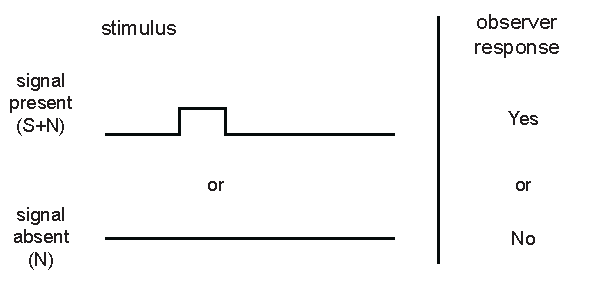
\includegraphics[scale=0.7]{figs/yesno.pdf}
\end{center}

{\small
\begin{columns}
\begin{column}{0.7\textwidth}

{\renewcommand{\arraystretch}{1.5}
\begin{tabular}{ rr|>{\centering\arraybackslash}p{2cm}|>{\centering\arraybackslash}p{2cm}| }
\multicolumn{1}{r}{} & \multicolumn{1}{r}{} & \multicolumn{2}{c}{Signal}\\
\multicolumn{1}{r}{} & \multicolumn{1}{r}{} &  \multicolumn{1}{c}{present}  & \multicolumn{1}{c}{absent} \\
\cline{3-4}
\multirow{2}{*}{Response} & Yes & Hit& False Alarm\\
\cline{3-4}
& No & Miss& Correct rejection\\
\cline{3-4}
\multicolumn{1}{r}{} & \multicolumn{1}{r}{} & \multicolumn{1}{r}{$N_s$} & \multicolumn{1}{r}{$N_n$}\\
\end{tabular}
}

\end{column}
\begin{column}{0.3\textwidth}

\begin{itemize}
\item Hit rate \\ $pH = \frac{\# H}{\# N_{s}}$
\item False Alarm rate \\ $pFA = \frac{\# FA}{\#N_{n}}$

\end{itemize}

\end{column}
\end{columns}
}
\end{frame}

%%
\begin{frame}
\textbf{Example}
\begin{columns}
\begin{column}{0.7\textwidth}

{\renewcommand{\arraystretch}{1.5}
\begin{tabular}{ rr|>{\centering\arraybackslash}p{2cm}|>{\centering\arraybackslash}p{2cm}| }
\multicolumn{1}{r}{} & \multicolumn{1}{r}{} & \multicolumn{2}{c}{Signal}\\
\multicolumn{1}{r}{} & \multicolumn{1}{r}{} &  \multicolumn{1}{c}{present}  & \multicolumn{1}{c}{absent} \\
\cline{3-4}
\multirow{2}{*}{Response} & Yes & 180 & 50\\
\cline{3-4}
& No & 20 & 150\\
\cline{3-4}
\multicolumn{1}{r}{} & \multicolumn{1}{r}{} & \multicolumn{1}{r}{200} & \multicolumn{1}{r}{200}\\
\end{tabular}
}

\end{column}
\begin{column}{0.3\textwidth}

\begin{itemize}
\item Hit rate \\ $pH = \frac{\# H}{\# N_{s}} = \frac{180}{200} = 0.9$ \\[10pt]
\item False Alarm rate \\ $pFA = \frac{\# FA}{\#N_{n}} = \frac{50}{200} = 0.25$

\end{itemize}

\end{column}
\end{columns}
\end{frame}

%%
\begin{frame}[fragile]{Exercise 1: Analyze a detection experiment}

\begin{tabular}{ll}
Datafile: & \textit{data1.csv}\\
Description: & columns are: \\
& Resp (response, 1: Yes, 0: No)\\
& Stim (type of stimulus, 'S': signal-present, 'A': signal-absent).
\end{tabular}
\vspace{10pt}
Steps:
\begin{enumerate}
\item Load \textit{data1.csv} as a dataframe in R using \begin{verbatim} read.csv()\end{verbatim}
\item Examine its contents with \begin{verbatim} head() summary() \end{verbatim}
\item Calculate Hit and False Alarm Rate ($pH$ and $pFA$)
\end{enumerate}
\vspace{10pt}
\textit{Hints: slicing the data in R can be done with square brackets ([ ]) and selecting a column is done with the dollar sign (\$)}
\pause
\begin{center}
$pH = 0.936$\\
$pFA = 0.288 $
\end{center}
\end{frame}



%%
\begin{frame}{Signal detection theory}

\begin{center}
\includegraphics<1>[scale=0.9]{figs/normaldist1.pdf}
\includegraphics<2>[scale=0.9]{figs/normaldist2.pdf}
\end{center}

\textbf{Assumptions:}
\begin{itemize}
\item Internal dimension representing some (sensory) evidence, $X$
\item subjected to fluctuation (noise), $X$ is a random var.
\item simple decision rule: if $X > c$ then respond $YES$\\
otherwise respond $NO$
\end{itemize}

\end{frame}


\subsection{Equal-variance, Gaussian SDT}
\begin{frame}{SDT with some added assumptions}

\begin{block}{1. Assumption of Gaussian distribution }
$X_n \sim \mathcal{N} (0, 1)$ and 
$X_s \sim \mathcal{N}(\mu_s, \sigma^2_s)$
\end{block}

\begin{block}{2. Equal-variance assumption}

even further simplification $\sigma^2_s =  1$
\end{block}

\begin{center}
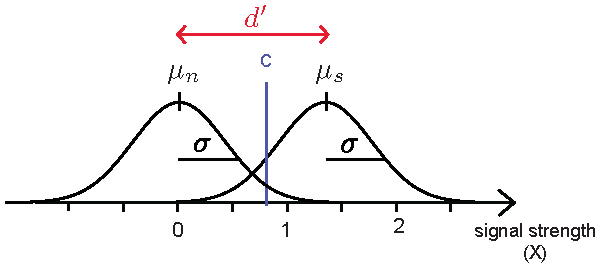
\includegraphics[scale=1]{figs/evgsdt.pdf}
\end{center}
\end{frame}

\begin{frame}{Equal-variance, Gaussian-distributed signal detection}
\begin{block}{It is then defined}
$d'$, a \textit{measure of sensitivity} defined as the distance between the two distributions\\
$c$ is the sensory criterion and a \textit{measure of bias}.
\end{block}


\begin{center}
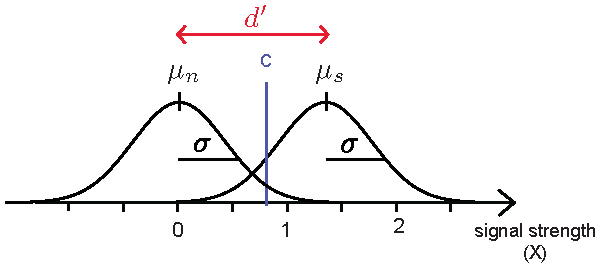
\includegraphics[scale=1]{figs/evgsdt.pdf}
\end{center}

\begin{center}
\vspace{20pt}
\textbf{Equal-variance, Gaussian-distributed signal detection is\\
the model most commonly used}
\end{center}
\end{frame}


%%
\begin{frame}{Equal-variance, Gaussian-distributed signal detection}

Parameters $d'$ and $c$ can be calculated directly from
$pH$ and $pFA$.\\

\begin{center}
\includegraphics<2->[scale=0.8]{figs/areas.pdf}
\includegraphics<1>[scale=0.8]{figs/areas2.pdf}
\end{center}

\only<2>{\centering $pH = 1 - \Phi(c - d')$}
\only<1>{\centering $pFA = 1 - \Phi(c)$}

\only<3->{
\begin{center}
$pFA = 1 - \Phi(c)$ \quad \quad $pH = 1 - \Phi(c - d')$
\end{center}

\begin{block}{it can be solved for $d'$ and $c$ {\scriptsize [full derivation in extra slides *1]}}
\begin{equation}
c = -\Phi^{-1}(pFA)
\label{eq:c}
\end{equation}
\begin{equation}
d'= \Phi^{-1}(pH) - \Phi^{-1}(pFA)
\label{eq:dp}
\end{equation}
\end{block}
}
\end{frame}


%% 
\begin{frame}{Exercise 2: explore the normal distribution}

\begin{enumerate}
\item Draw 1000 random samples from a (standard) normal distribution ($\mu_0, \sigma^2=1$). Save in a vector $x$
\item Plot the histogram of $x$
\item Plot a cumulative histogram: plot the cumulative sum against the histogram bins.
\item Plot the inverse of it
\item Relate the functions $qnorm()$ and $pnorm()$ with these obtained plots
\end{enumerate}
\end{frame}


%%
\begin{frame}{}
$\Phi()$ is the cumulative normal dist. function\\
and $\Phi^{-1}()$ its inverse, or \textit{quantile} function


\begin{center}
\includegraphics[scale=0.5]{figs/linkfun.pdf}
\end{center}
\end{frame}

%%
\begin{frame}[fragile]{Exercise 3: Analyze a detection experiment}
\begin{enumerate}
\item Use the Eqs. to calculate $d'$ and $c$.
\end{enumerate}

\begin{block}{}
\begin{equation*}
c = -\Phi^{-1}(pFA)
\end{equation*}
\begin{equation*}
d'= \Phi^{-1}(pH) - \Phi^{-1}(pFA)
\end{equation*}
\end{block}

\pause
\begin{verbatim}
> dp_hat <- qnorm(pH) - qnorm(pFA)
2.081273
> c_hat <- -qnorm(pFA)
0.559237
\end{verbatim}

\begin{center}
$\hat{d'} = 2.081273$\\
$\hat{c} = 0.559237$
\end{center}

\end{frame}

%%
\begin{frame}[fragile]{Exercise 3': Analyze a detection experiment}
Some textbooks use the calculation of a modified criterion $c_{center} = C$ that is midway between the two distributions

\begin{align*}
C = c_{center} & = -\Phi^{-1}(pH) + d'/2 = -\Phi^{-1}(pFA) - d'/2 \\
& = -[\Phi^{-1}(pH) + \Phi^{-1}(pFA)]/2 
\end{align*}

\begin{center}
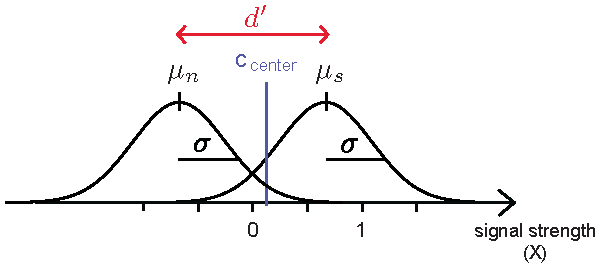
\includegraphics[scale=0.8]{figs/c_center.pdf}
\end{center}

\pause
\begin{verbatim}
> c_center <- -(qnorm(pH) + qnorm(pFA))/2.0
-0.4813996
\end{verbatim}


\end{frame}

%%
\section{Generalized Linear Models}
\begin{frame}{Generalized Linear Models (GLMs)}
Another approach to estimate $\hat{d'}$ and $\hat{c}$ is using GLMs.\\[5pt]

A GLM is a linear model generalized for response variables that are not necessarily continuous. 

Let's consider a linear model
\begin{center}
$y = \beta_1 \cdot x + \beta_0$
\end{center}

GLMs made linear models \textbf{general} by having $y$ replaced by a probability value (the expectation of Y, $E[Y]$), and adding a function $g()$ that 'links' the linear predictors (right-hand side) with the probability in the response variable.

\begin{center}
$g(E[y])= \beta_1 \cdot x + \beta_0$
\end{center}

There could be  explanatory variables ($\beta_0, \beta_1, \beta_2 \dots$), therefore GLMs are  annotated in a vector form 

$$
g(E[\mathbf{Y}]) = \mathbf{X} \cdot \mathbf{\beta}
$$

\end{frame}



%%
\subsection{GLMs and SDT}
%
\begin{frame}{GLM and SDT}
Note that the False Alarm and Hit Rates are probabilities

$$ pFA = P[R=YES| S=absent] = P[Y=1 | X=0] $$
$$ pH =P[R=YES | S=present] = P[Y=1 | X=1] $$

Thus, one could write 
$$g(P[Y=1]) = \beta_1 \cdot X + \beta_0 $$

\hfill where \\
\hfill $X=1$ for signal-present trials and \\
\hfill $X=0$ for signal-absent trials.

\end{frame}


%%
\begin{frame}{GLM and SDT}
Let's consider our detection experiment. The GLM for a detection experiment can be arranged
\begin{align*}
g(E[\mathbf{Y}]) &= \mathbf{X} \cdot \mathbf{\beta}\\
    g( 
    \begin{bmatrix}
           0 \\
           1 \\
           0 \\
           \vdots \\
           1 \\
           1 \\
           1 \\
    \end{bmatrix} ) &= 
    \begin{bmatrix}
           1 & 0 \\
           1 & 0 \\
           1 & 0 \\
           \vdots \\
           1 & 1 \\
           1 & 1 \\
           1 & 1 \\
    \end{bmatrix} \cdot
    \begin{bmatrix}
           \beta_0 \\
           \beta_1 
    \end{bmatrix}
\end{align*}

The first set of responses correspond to signal-absent trials, and the second set to signal-present trials. \\
This GLM can be then solved using maximum likelihood estimation (MLE).\\
The procedure returns estimates for $\beta_0$ and $\beta_1$.


\end{frame}


%%
\begin{frame}{Link function $g()$}
For this case an appropriate choice of the link function is the quantile normal function $g() = \Phi^{-1}()$

\begin{center}
\includegraphics[scale=0.5]{figs/linkfun.pdf}
\end{center}

\end{frame}

%%
\begin{frame}[fragile]{Exercise 4: Analyze a detection experiment using a GLM}
\begin{enumerate}
\item Use the \textit{GLM method} to analyse the detection experiment data\\
\end{enumerate}

\pause
\begin{verbatim}
> fit <- glm(Resp ~ Stim, data=df, 
                     family=binomial('probit'))
\end{verbatim}
\end{frame}


%%
\begin{frame}[fragile]{}
\begin{verbnobox}[\small]
> summary(fit)
Call:
glm(formula = Resp ~ Stim, family = binomial("probit"), data = df)

Deviance Residuals: 
    Min       1Q   Median       3Q      Max  
-2.3447  -0.8242   0.3637   0.3637   1.5778  

Coefficients:
            Estimate Std. Error z value Pr(>|z|)    
(Intercept) -0.55924    0.05935  -9.422   <2e-16 ***
StimS        2.08127    0.10563  19.704   <2e-16 ***
---
Signif. codes:  0 ‘***’ 0.001 ‘**’ 0.01 ‘*’ 0.05 ‘.’ 0.1 ‘ ’ 1

(Dispersion parameter for binomial family taken to be 1)

    Null deviance: 1335.69  on 999  degrees of freedom
Residual deviance:  838.19  on 998  degrees of freedom
AIC: 842.19

Number of Fisher Scoring iterations: 5
\end{verbnobox}

\begin{center}
Do these numbers look familiar? \\
$\beta_1 = 2.08127$ and $\beta_0 = -0.55924 $
\end{center}
\end{frame}

%%
\begin{frame}{Explanation to the meaning of $\beta_0$ and $\beta_1$}
\begin{block}{Remember from before}
\begin{center}
$d'= \Phi^{-1}(pH) - \Phi^{-1}(pFA)$ \\
$c = -\Phi^{-1}(pFA)$
\end{center}
\end{block}

\only<1>{
For \textbf{signal-absent} trials, $X=0$  and the expanded model is
\begin{align*}
g(P[Y=1|X=0]) & = \beta_1 \cdot 0 + \beta_0  \\
\Phi^{-1}(P[Y=1|X=0]) & = \beta_0  \\
\Phi^{-1}(pFA) & = \beta_0  \\
-c & = \beta_0  
\end{align*}
}
\only<2->{
For \textbf{signal-present} trials, $X=1$  and the expanded model is
\begin{align*}
g(P[Y=1|X=1]) & = \beta_1 \cdot 1 + \beta_0  \\
\Phi^{-1}(P[Y=1|X=1]) & = \beta_1 \cdot 1 + \Phi^{-1}(pFA)   \\
\Phi^{-1}(pH) & = \beta_1 + \Phi^{-1}(pFA)   \\
\Phi^{-1}(pH) - \Phi^{-1}(pFA) & = \beta_1\\
d' & = \beta_1\\
\end{align*}

{\small Therefore, the coefficients obtained from GLM have a direct correspondence to the parameters $d'$ and $c$. }
}
\end{frame}

%%
\begin{frame}[fragile]{The power of GLMs}
\textbf{Confidence intervals}
\begin{verbatim}
> confint(fit)
Waiting for profiling to be done...
                 2.5 %     97.5 %
(Intercept) -0.6761901 -0.4434893
StimS        1.8773729  2.2917211
\end{verbatim}


\end{frame}


\subsection{Conditions and model comparison with GLMs}
%%
\begin{frame}[fragile]{Exercise 5: Detection exp. in two conditions}

To include different conditions in the GLM framework \\[10pt]

\textbf{Reading data from two exp. conditions}
\begin{verbatim}
> df1 <- read.csv("data1.csv")
> df1$Cond <- "A"

> df2 <- read.csv("data2.csv")
> df2$Cond <- "B"

> df <- rbind(df1, df2)
\end{verbatim}
\end{frame}

%%
\begin{frame}[fragile]{Exercise 5: Detection exp. in two conditions}
\textbf{Fitting different models}\\[10pt]
\textit{(a) Unique model}
\begin{verbatim}
> fit1 <- glm(Resp ~ Stim, 
        family=binomial('probit'), data=df)
\end{verbatim}

\textit{(b) Model with different criteria, same sensitivity ($d'$)}
\begin{verbatim}
> fit2 <- glm(Resp ~ Stim + Cond, 
         family=binomial('probit'), data=df)
\end{verbatim}

\textit{(c) Model with different criteria and sensitivity ($d'$)}
\begin{verbatim}
> fit3 <- glm(Resp ~ Stim + Cond + Stim:Cond, 
         family=binomial('probit'), data=df)
\end{verbatim}

\end{frame}



%% 
\begin{frame}{Design matrix}
$$
g(E[\mathbf{Y}]) = \mathbf{X} \cdot \mathbf{\beta}
$$

\begin{itemize}
\item The design matrix $X$ is automatically generated by $R$.
\item It can always be obtained using the function $model.matrix()$
\end{itemize}
\end{frame}



%%
\begin{frame}[fragile]{Understanding the design matrix}

For the unique model (a), the GLM  looks like 
\begin{align*}
g(E[\mathbf{Y}]) &= \mathbf{X} \cdot \mathbf{\beta}\\
    g( 
    \begin{bmatrix}
           0 \\
           1 \\
           \vdots \\
           1 \\
           1 \\
           \vdots \\
           1 \\
           0 \\
           \vdots \\
           1 \\
           1 \\
    \end{bmatrix} ) &= 
    \begin{bmatrix}
           1 & 0 \\
           1 & 0 \\
           \vdots \\
           1 & 1 \\
           1 & 1 \\
           \vdots \\
           1 & 0 \\
           1 & 0 \\
           \vdots \\
           1 & 1 \\
           1 & 1 \\
    \end{bmatrix} \cdot
    \begin{bmatrix}
           \beta_0 \\
           \beta_1 
    \end{bmatrix}
\end{align*}

\end{frame}



%%
\begin{frame}[fragile]{Understanding the design matrix}
For the model(b): different intercept ($fit2$), the GLM looks like 
\begin{align*}
g(E[\mathbf{Y}]) &= \mathbf{X} \cdot \mathbf{\beta}\\
    g( 
    \begin{bmatrix}
           0 \\
           1 \\
           \vdots \\
           1 \\
           1 \\
           \vdots \\
           1 \\
           0 \\
           \vdots \\
           1 \\
           1 \\
    \end{bmatrix} ) &= 
    \begin{bmatrix}
           1 & 0 & 0 \\
           1 & 0  & 0 \\
           \vdots \\
           1 & 1 & 0 \\
           1 & 1 & 0 \\
           \vdots \\
           1 & 0 & 1 \\
           1 & 0 & 1 \\
           \vdots \\
           1 & 1 & 1 \\
           1 & 1 & 1 \\
    \end{bmatrix} \cdot
    \begin{bmatrix}
           \beta_0 \\
           \beta_1 \\
           \beta_2 
    \end{bmatrix}
\end{align*}
{\small \hfill see [*2] for full derivation of parameters}
\end{frame}


%%
\begin{frame}[fragile]{Understanding the design matrix}
For the model (c): different intercept and different d' ($fit3$), the GLM looks like 

\begin{align*}
g(E[\mathbf{Y}]) &= \mathbf{X} \cdot \mathbf{\beta}\\
    g( 
    \begin{bmatrix}
           0 \\
           1 \\
           \vdots \\
           1 \\
           1 \\
           \vdots \\
           1 \\
           0 \\
           \vdots \\
           1 \\
           1 \\
    \end{bmatrix} ) &= 
    \begin{bmatrix}
           1 & 0 & 0 & 0\\
           1 & 0 & 0 & 0\\
           \vdots \\
           1 & 1 & 0 & 0\\
           1 & 1 & 0 & 0\\
           \vdots \\
           1 & 0 & 1 & 0\\
           1 & 0 & 1 & 0\\
           \vdots \\
           1 & 1 & 1 & 1\\
           1 & 1 & 1 & 1\\
    \end{bmatrix} \cdot
    \begin{bmatrix}
           \beta_0 \\
           \beta_1 \\
           \beta_2 \\
           \beta_3 
    \end{bmatrix}
\end{align*}
{\small \hfill see [*3] for full derivation of parameters}
\end{frame}



%%
\begin{frame}[fragile]{Exercise 5: Detection exp. in two conditions}
\textit{Model selection}

\begin{verbatim}
> anova(fit1, fit2, fit3, test='Chisq')
Analysis of Deviance Table

Model 1: Resp ~ Stim
Model 2: Resp ~ Stim + Cond
Model 3: Resp ~ Stim + Cond + Stim:Cond
  Resid. Df Resid. Dev Df Deviance  Pr(>Chi)    
1      1998     1735.5                          
2      1997     1701.8  1   33.698 6.435e-09 ***
3      1996     1701.7  1    0.140    0.7081    
---
Signif. codes:  0 ‘***’ 0.001 ‘**’ 0.01 ‘*’ 0.05 ‘.’ 0.1 ‘ ’ 1
\end{verbatim}



\alert{fit2 explains the data sig. better than fit1, but fit3 does not improve it further}
\end{frame}

%%
\begin{frame}[fragile]{Exercise 5: Detection experiment on two conditions}
\textit{Parameter extraction}
\begin{verbatim}
> coef(fit2)
(Intercept)       StimS       CondB 
 -0.5500044   2.0521900  -0.3999372 
\end{verbatim}

How are these parameters encoded?\\[10pt]
\pause
Remember from earlier that $\beta_0 = -c$ and $\beta_1 = d'$\\[5pt]

\begin{itemize}
\item The intercept applies for the first condition ($A$), thus
$\beta_0 = -c_A$.
\item $\beta_1 = d'$, assumed equal for both conditions A and B.
\item The new parameter $\beta_2$ is the difference with respect to $\beta_0$. Thus, $c_B = - (\beta_0 + \beta_2)$.
\end{itemize}

Thus,
\begin{verbatim}
> c_b <- -(coef(fit2)[[1]]+coef(fit2)[[3]])
0.9499416
\end{verbatim}
\end{frame}



%%
\section{Discrimination Experiment: 2-AFC}
\begin{frame}{Discrimination Experiment: 2-AFC}

\begin{center}
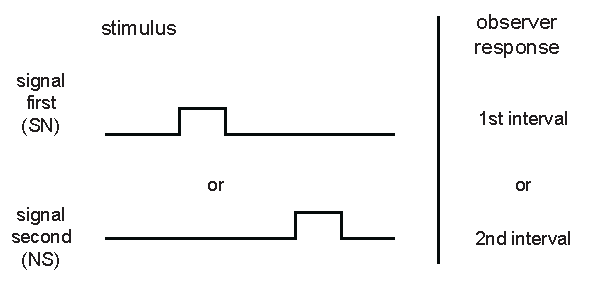
\includegraphics[scale=0.75]{figs/2afc_design.pdf}
\end{center}

\begin{itemize}
\item Statistically similar as in a Yes/No detection experiment
\item Signal-present or -absent can be relabeled to 'SN'/'NS'
and responses as '1st interval'/'2nd interval', or  '1st position'/'2nd position'
depending on the exp. design
\item Extra step of differencing
\end{itemize}
\end{frame}


%%
\begin{frame}{Discrimination Experiment: 2-AFC}
\textbf{On each trial, two stimuli are presented}. Thus, two draws are taken, one from each distribution

\begin{center}
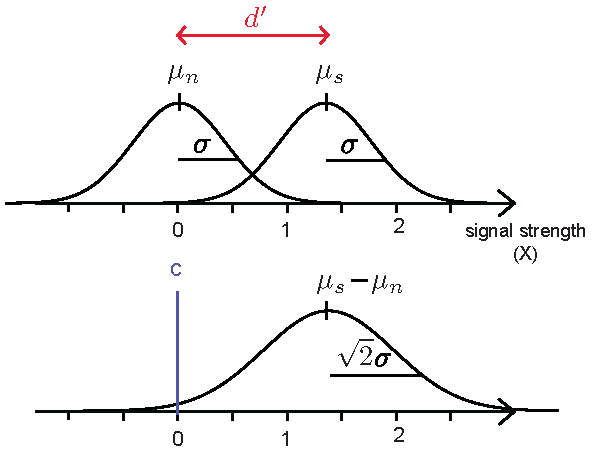
\includegraphics[scale=0.7]{figs/2afc.pdf}
\end{center}

$$
\Delta = X_s - X_n \quad \quad \Delta \sim \mathcal{N} (\mu_s - \mu_n, 2\sigma^2)
$$

\end{frame}

%%
\begin{frame}{Discrimination Experiment: 2-AFC}

$$
\Delta = X_s - X_n \quad \quad \Delta \sim \mathcal{N} (\mu_s - \mu_n, 2\sigma^2)
$$
As $\mu_n=0$, $\mu_s=d'$, and $\sigma=1$, we have

$$
\Delta \sim \mathcal{N} (d', 2)
$$
and the probability of correct  when $\Delta > 0$,

$$Pc = 1 -\Phi\left(\frac{-d'}{\sqrt{2}}\right) = \Phi\left(\frac{d'}{\sqrt{2}} \right)
$$

Thus, $d'$ can be calculated from the percentage correct in a 2-AFC experiment

\begin{equation}
\label{eq:dp_2afc}
d' = \Phi^{-1}(Pc) \sqrt{2}
\end{equation}

\end{frame}

%%
\begin{frame}{Discrimination Experiment: 2-AFC}

Estimates of d' from 2AFC and Yes/No related to each other by 
$$
d'_{AFC} =  d'_{YesNo} \sqrt{2}
$$ 

(see derivation in Wickens 2002,  or in McNicol 1972 )\\
\vspace{30pt}

However, this relationship has been called into question recently (Yeshurun, Carrasco \& Maloney, 2008)
\end{frame}




%%
\begin{frame}[fragile]{Exercise 6: Discrimination experiment: 2-AFC}

Analyze the data from a 2-AFC discrimination experiment using a GLM

\begin{tabular}{ll}
Datafile: & \textit{datatwoafc.csv}\\
Description: & columns are: \\
& Resp (response, 1: 1st interval, 0: 2nd interval)\\
& Stim (type of stimulus, 'SN': stimulus in 1st interval, \\
& or 'NS': stimulus in 2nd interval).
\end{tabular}

\vspace{10pt}


Steps:
\begin{enumerate}
\item Load data
\item Calculate percentage correct $Pc$ and from it $d'$ using Eq. \autoref{eq:dp_2afc}
\item Calculate $d'$ and $c$ using a GLM
\item Compare these two ways of obtaining $d'$
\end{enumerate}

\pause
\begin{center}
Solution: $d' = 1.53$, $c=0.77$, $c_{center} = 0.01$
\end{center}
\end{frame}



%%
\section{Further Exercises}
\begin{frame}{Further Exercises}

\begin{itemize}

\item \textbf{Exercise 7}: Add to the analysis in Exercise 5 (Yes/No experiment) two other conditions: \textit{data3.csv} and \textit{data4.csv}. \\
Does d' change across all four conditions?

\vspace{20pt}
\item \textbf{Exercise 8}: Analyse another Yes/No experiment in two conditions: \textit{data\_small\_1.csv} and \textit{data\_small\_2.csv}. This time the experiment was done with a small number of trials.\\
Does d' change between these two conditions?


\vspace{20pt}
\item \textbf{Exercise 9}: Analyze the data of a 2-AFC experiment in two conditions: \textit{datatwoafc-2.csv} and \textit{datatwoafc-3.csv}\\
Test a model for a change in sensitivity between these two conditions.


\end{itemize}

\end{frame}



%%%%%%%%%%%%%%%%%%%%%%%%%%%%%%%%%%%%%%%%%%%%%%%%%%%%%%%%%%%%%%%%%%%%%%
\section{MLDS}
\begin{frame}{Maximum Likelihood Difference Scaling}
Scaling method aimed to find $\Psi(x)$
\begin{center}
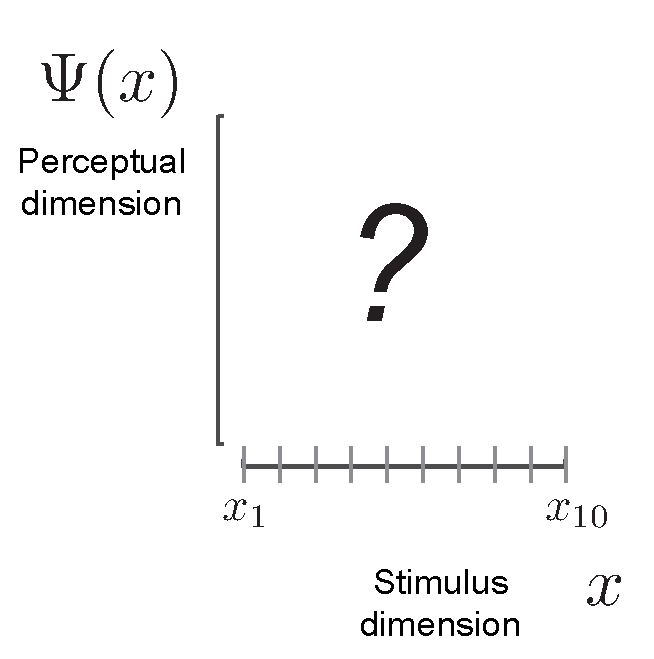
\includegraphics[width=0.5\textwidth]{figs/scaling_stimspacing.pdf}
\end{center}
\end{frame}


%%
\begin{frame}{Maximum Likelihood Difference Scaling (MLDS)}
\begin{center}
Task: \textit{Which pair is more different?}

\vspace{10pt}
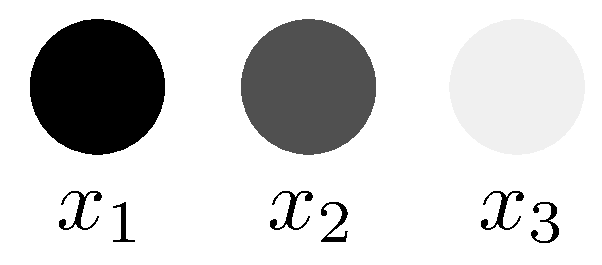
\includegraphics[scale=0.4]{figs/triad.pdf}\\
%{\small \textit{method of triads}}
%\vspace{10pt}
\begin{block}{Decision model}
\begin{align*}
\Delta & = [\Psi (x_3) - \Psi (x_2)] - [\Psi (x_2) - \Psi (x_1)] + \epsilon\\
& = \Psi (x_3) - 2 \Psi (x_2) + \Psi (x_1) + \epsilon  \quad \quad \quad \quad \quad \quad \quad \quad \epsilon \sim \mathcal{N}(0, \sigma^2)
\end{align*}
\begin{align*}
\text{if} \, \Delta>0 & \rightarrow (x_2, x_3)\\
\text{otherwise} & \rightarrow (x_1, x_2)
\end{align*}
\end{block}
\end{center}
\end{frame}


%%
\begin{frame}{Maximum Likelihood Difference Scaling (MLDS)}
\begin{adjustwidth}{-2em}{-2em}
\begin{center}
MLDS uses a Generalized Linear Model (GLM) to find $\Psi(x)$\\[10pt]

\includegraphics<1-2>[scale=0.4]{figs/figure3_stripped_1.pdf}
\includegraphics<3-4>[scale=0.4]{figs/figure3_stripped_2.pdf}
\includegraphics<5>[scale=0.4]{figs/figure3_stripped.pdf}
\end{center}

\only<1>{
\begin{align*}
\Delta & = \Psi(x_2) - 2 \Psi(x_5) + \Psi(x_8)\\
\end{align*}
}

\only<2-3>{
\begin{align*}
\Delta & = \Psi(x_2) - 2 \Psi(x_5) + \Psi(x_8) + \epsilon\\
g(E[Y]) & = \boldsymbol{1} \cdot \beta_2 - \boldsymbol{2} \cdot \beta_5 + \boldsymbol{1} \cdot \beta_8  + \epsilon\\
& \qquad \qquad \hdots
\end{align*}
}
%g(P[Y=1]) & = 1 \cdot \beta_3 - 2 \cdot \beta_8 + 1 \cdot \beta_9  \quad + \epsilon\\
\only<4-5>{
{\small
\begin{center}
\begin{itemize}
\item[] $\boldsymbol{Y}$: vector of observer responses (binary)
\item[] $\boldsymbol{X}$: design matrix
\item[] $\boldsymbol{\beta}$: GLM coefficients $\rightarrow$ perceptual scale
\item[] $g()$: link function
\end{itemize}
\end{center}

}
}
\end{adjustwidth}
\end{frame}



%%
\begin{frame}[fragile]{Exercise 10: Estimate a perceptual scale using MLDS}

Analyze the data from a MLDS scaling experiment

\begin{tabular}{ll}
Datafile: & \textit{datamlds.csv}\\
Description: & columns are: \\
& Resp (response, 0: 1st pair (x1, x2), 1: 2nd pair (x2, x3) \\
& s1, s2, s3: Stimulus values on each triad\\
\end{tabular}

\vspace{10pt}

Steps:
\begin{enumerate}
\item Load data
\item Explore the data with $head()$ and $summary()$
\item Calculate the perceptual scale using the function $mlds()$, from package $MLDS$ (package needs to be installed).
\end{enumerate}

\end{frame}


%%%%%%%%%%%%%%%%%%%%%%%%%%%%%%%%%%%%%%%%%%%%%%%%%%%%%%%%%%%%%%%%%%%%
\begin{frame}
\begin{center}
{\Huge Thank you}
\end{center}
\end{frame}

\section{Appendix: some mathematical derivations}
\begin{frame}{*1: Derivation 1}
\begin{center}
Given $pFA = 1 - \Phi(c)$ and $pH = 1 - \Phi(c - d')$

\begin{align*}
\Phi(c) & = 1 - pFA & \Phi(c - d') & = 1 - pH\\
c & = \Phi^{-1}(1 - pFA) & c - d' & = \Phi^{-1}(1 - pH) \\
c & = -\Phi^{-1}(pFA)  &  d' & = c - \Phi^{-1}(1 - pH)  \\
& & d' & = -\Phi^{-1}(pFA)  - \Phi^{-1}(1 - pH) \\
& & d' & = \Phi^{-1}(pH) - \Phi^{-1}(pFA)\\
\end{align*}

Note the symmetry of the quantile function\\
$\Phi^{-1}(1-x) = -\Phi^{-1}(x)$
\end{center}
\end{frame}


\begin{frame}{*2: Derivation 2}
For the model(b): different intercept ($fit2$), the GLM looks like 
\begin{align*}
g(E[\mathbf{Y}]) &= \mathbf{X} \cdot \mathbf{\beta}\\
    g( 
    \begin{bmatrix}
           0 \\
           1 \\
           \vdots \\
           1 \\
           1 \\
           \vdots \\
           1 \\
           0 \\
           \vdots \\
           1 \\
           1 \\
    \end{bmatrix} ) &= 
    \begin{bmatrix}
           1 & 0 & 0 \\
           1 & 0  & 0 \\
           \vdots \\
           1 & 1 & 0 \\
           1 & 1 & 0 \\
           \vdots \\
           1 & 0 & 1 \\
           1 & 0 & 1 \\
           \vdots \\
           1 & 1 & 1 \\
           1 & 1 & 1 \\
    \end{bmatrix} \cdot
    \begin{bmatrix}
           \beta_0 \\
           \beta_1 \\
           \beta_2 
    \end{bmatrix}
\end{align*}
\end{frame}

%%
\begin{frame}{*2: Derivation 2}
Writing each case we have 
\begin{align*}
g(E[Y=1| X=0, C=A]) & = 1* \beta_0 + 0 * \beta_1 + 0* \beta_2 \\
g(E[Y=1| X=1, C=A]) & = 1* \beta_0 + 1 * \beta_1 + 0* \beta_2 \\
g(E[Y=1| X=0, C=B]) & = 1* \beta_0 + 0 * \beta_1 + 1* \beta_2 \\
g(E[Y=1| X=1, C=B]) & = 1* \beta_0 + 1 * \beta_1 + 1* \beta_2 \\
\end{align*}

by replacing expectations for FA and Hit Rates, and by replacing the link function for the quantile function $g() = \Phi^{-1}()$, we have

\begin{align}
\Phi^{-1}(pFA_{A}) & = \beta_0 \label{eq:1}\\
\Phi^{-1}(pH_{A}) & = \beta_0 + \beta_1 \label{eq:2}\\
\Phi^{-1}(pFA_{B}) & = \beta_0 + \beta_2  \label{eq:3}\\
\Phi^{-1}(pH_{B}) & = \beta_0 + \beta_1 + \beta_2 \label{eq:4}
\end{align}
\end{frame}

%%
\begin{frame}{*2: Derivation 2}
Simplifying Eq. \autoref{eq:1}, 
\begin{align*}
\beta_0 & = \Phi^{-1}(pFA_{A}) = -c_A \quad \quad \quad c_A = -\beta_0\\
\end{align*}

inserting $\beta_0$ in Eq. \autoref{eq:2}...
\begin{align*}
\Phi^{-1}(pH_{A}) & = \Phi^{-1}(pFA_{A}) + \beta_1\\
\Phi^{-1}(pH_{A}) - \Phi^{-1}(pFA_{A}) & =  \beta_1\\
d' & = \beta_1 \\
\end{align*}

Then, Eq. \autoref{eq:3}..
\begin{align*}
\Phi^{-1}(pFA_{B}) & = \beta_0  + \beta_2 \\
\Phi^{-1}(pFA_{B}) - \beta_0 & =  \beta_2 \\
- c_B + c_A & =  \beta_2 \\
- (c_B - c_A) & =  \beta_2 \\
\end{align*}
\end{frame}

\begin{frame}{*2: Derivation 2}

$\beta_2$ is the difference in intercept between conditions B and A\\

\vspace{10pt}

Finally inserting $\beta_0, \beta_1, \beta_2$ in Eq. \autoref{eq:4} ..
\begin{align*}
\Phi^{-1}(pH_{B}) = & \beta_0 + \beta_1 + \beta_2\\
\Phi^{-1}(pH_{B}) = & \Phi^{-1}(pFA_{A}) + \Phi^{-1}(pH_{A}) - \Phi^{-1}(pFA_{A}) \\
& + \Phi^{-1}(pFA_{B}) - \Phi^{-1}(pFA_{A})\\
\Phi^{-1}(pH_{B}) = & \Phi^{-1}(pH_{A}) + \Phi^{-1}(pFA_{B}) - \Phi^{-1}(pFA_{A})\\
\Phi^{-1}(pH_{B}) - \Phi^{-1}(pFA_{B}) = & \Phi^{-1}(pH_{A}) - \Phi^{-1}(pFA_{A})\\
d'_B = & d'_A\\
\end{align*}
\end{frame}


%%
\begin{frame}{*3: Derivation 3}
Writing each case we have 
\begin{align*}
g(E[Y=1| X=0, C=A]) & = 1* \beta_0 + 0 * \beta_1 + 0* \beta_2 +  0* \beta_3 \\
g(E[Y=1| X=1, C=A]) & = 1* \beta_0 + 1 * \beta_1 + 0* \beta_2 +  0* \beta_3 \\
g(E[Y=1| X=0, C=B]) & = 1* \beta_0 + 0 * \beta_1 + 1* \beta_2 +  0* \beta_3 \\
g(E[Y=1| X=1, C=B]) & = 1* \beta_0 + 1 * \beta_1 + 1* \beta_2 +  1* \beta_3 \\
\end{align*}

by replacing expectations for FA and Hit Rates, and by replacing the link function for the quantile function $g() = \Phi^{-1}()$, we have

\begin{align}
\Phi^{-1}(pFA_{A}) & = \beta_0 \label{eq:c1}\\
\Phi^{-1}(pH_{A}) & = \beta_0 + \beta_1 \label{eq:c2}\\
\Phi^{-1}(pFA_{B}) & = \beta_0 + \beta_2  \label{eq:c3}\\
\Phi^{-1}(pH_{B}) & = \beta_0 + \beta_1 + \beta_2 +  \beta_3\label{eq:c4}
\end{align}
\end{frame}

%%
\begin{frame}{*3: Derivation 3}
Simplifying Eq. \autoref{eq:c1}, 
$$
\beta_0  = \Phi^{-1}(pFA_{A}) = -c_A
$$

inserting $\beta_0$ in Eq. \autoref{eq:c2}...
\begin{align*}
\Phi^{-1}(pH_{A}) & = \Phi^{-1}(pFA_{A}) + \beta_1\\
\Phi^{-1}(pH_{A}) - \Phi^{-1}(pFA_{A}) & =  \beta_1\\
d'_A & = \beta_1 \\
\end{align*}

inserting $\beta_0$ in Eq. \autoref{eq:c3} ..
\begin{align*}
\Phi^{-1}(pFA_{B}) & = \Phi^{-1}(pFA_{A})  + \beta_2 \\
\Phi^{-1}(pFA_{B}) - \Phi^{-1}(pFA_{A}) & =  \beta_2 \\
- (c_B - c_A) & =  \beta_2 \\
\end{align*}
$\beta_2$ is the difference in intercept between conditions B and A\\
\end{frame}

\begin{frame}{*2: Derivation 2}

Finally inserting $\beta_0, \beta_1, \beta_2$ in Eq. \autoref{eq:c4} ..
\begin{align*}
\Phi^{-1}(pH_{B}) = & \beta_0 + \beta_1 + \beta_2 + \beta_3\\
\Phi^{-1}(pH_{B}) = & \Phi^{-1}(pFA_{A}) + \Phi^{-1}(pH_{A}) - \Phi^{-1}(pFA_{A}) \\
& + \Phi^{-1}(pFA_{B}) - \Phi^{-1}(pFA_{A}) + \beta_3\\
\Phi^{-1}(pH_{B}) = & \Phi^{-1}(pH_{A}) + \Phi^{-1}(pFA_{B}) - \Phi^{-1}(pFA_{A}) + \beta_3\\
\Phi^{-1}(pH_{B}) - \Phi^{-1}(pFA_{B}) = & \Phi^{-1}(pH_{A}) - \Phi^{-1}(pFA_{A}) + \beta_3\\
d'_B = & d'_A + + \beta_3\\
d'_B - d'_A = & \beta_3\\
\end{align*}
$\beta_3$ is the difference in  $d'$ between conditions B and A
\end{frame}

\end{document}


